\documentclass[12pt]{article}
\usepackage[english, russian]{babel}
%\usepackage{makecell}
%\usepackage{multirow}
%\usepackage{hhline}
\usepackage{ulem}
\usepackage{minted}
\usepackage[TS1, T2A]{fontenc}
\usepackage[utf8]{inputenc}
\usepackage{hyperref}
\usepackage{dirtree}
\usepackage{graphicx}
%\def\dontdofcolorbox{\renewcommand\fcolorbox[4][]{##4}}
%\makeatother
\usepackage[left=2cm,right=2cm, top=1cm,bottom=1.5cm,bindingoffset=0cm]{geometry}

%\usepackage{multicol}
%\usepackage{dirtree} 
%\usepackage{graphicx}
%\graphicspath{{imgs/}}
%\DeclareGraphicsExtensions{.pdf,.png,.jpg}
\begin{document}
\setlength{\parindent}{0pt}
\pagestyle{empty}
\begin{center}
\normalsize
\textbf{Федеральное государственное автономное образовательное учреждение высшего образования}

\small
\medskip 
\textbf{САНКТ-ПЕТЕРБУРГСКИЙ НАЦИОНАЛЬНЫЙ ИССЛЕДОВАТЕЛЬСКИЙ  УНИВЕРСИТЕТ ИНФОРМАЦИОННЫХ ТЕХНОЛОГИЙ, МЕХАНИКИ И ОПТИКИ}

\medskip 
\textbf{ФАКУЛЬТЕТ ПРОГРАММНОЙ ИНЖЕНЕРИИ И КОМПЬЮТЕРНОЙ ТЕХНИКИ}
\end{center}
\bigskip\bigskip\bigskip\bigskip\bigskip\bigskip\bigskip\bigskip\bigskip\bigskip\bigskip\bigskip
\begin{center}
\par\medskip\par\smallskip
\Large
 
\par\smallskip
\textbf{ОТЧЕТ} 

\textbf{ПО ЛАБОРАТОРНОЙ РАБОТЕ №2}

\large
\par\bigskip
\textbf{«Языки системного программирования: \\ Использование ассемблерных вставок в языках высого уровня»}
\par\bigskip\par\bigskip\par\bigskip\par\bigskip\par\bigskip\par\bigskip
\par\bigskip\par\bigskip\par\bigskip\par\bigskip\par\bigskip\par\bigskip
\par\bigskip\par\bigskip\par\bigskip\par\bigskip\par\bigskip\par\bigskip
\end{center}
\begin{center}
\begin{tabular}{lllll}
Проверил:	 	 						& \hspace{80pt}	&	Выполнил:										&\\
Сентерев Ю.А.	 \_\_\_\_\_\_\_\_\_\_	&			    &	Студент группы P3255							&\\
«\_\_\_\_\_\_» 	 \_\_\_\_\_\_\_ 201\_г.  & 				&	Кабардинов Д. В. \_\_\_\_\_\_\_\_\_\_\_			&\\
										&				&													&\\
Оценка\hspace{12pt}\_\_\_\_\_\_\_\_\_	&				&													&\\
\end{tabular}
\par\bigskip\par\bigskip\par\bigskip
                                                  
\par\bigskip \par\bigskip
\end{center}
\par\bigskip\par\bigskip\par\bigskip\par\bigskip\par\bigskip\par\bigskip\par\bigskip\par\bigskip
\begin{center}
Санкт-Петербург
\par\bigskip
2019
\end{center}
\pagebreak
\textbf{Задание:} \\
Составить программу на языке С, использующую ассемблерную вставку \\
\par

\textbf{Цель работы:} \\
Рассмотреть на примере языка С, как можно использовать ассемблерные вставки в программах, написанных на языках высокого уровня \\

\textbf{Ход выполнения работы}\\
Ассемблерные  вставки  используются  для  «насильственного»  размещения  в  Си
-
программах 
ассемблерного кода, явно заданного программистом. Содержимое ассемблерной вставки никак компилятором не анализируется, но имеется возможность описать то, как это содержимое взаимодействует с переменными Си - программы и как изменятся регистры после выполнения этого ассемблерного кода.

Синтаксис оператора ассемблерной вставки следующий:\\
\_\_asm\_\_  (вставка : \textit{\textbf{список\_выходных\_операндов}} : \textit{\textbf{список\_входныx\_операндов}} : \textit{\textbf{список\_разрушаемых\_регистров}} ); \\
Начинается оператор ассемблерной вставки с ключевого слова $asm$ или 
\_\_asm\_\_, после чего в круглых скобках следует ее описание. 
вставка представляет собой строковую константу с ассемблерными инструкциями. \\ 
В теле вставки могут находиться  не только ассемблерные инструкции,  но  и  вообще любые  директивы, распознаваемые ассемблером gas.  В  частности,  это  позволяет изменить  используемый  им синтаксис инструкций по-умолчанию.
\begin{flushleft}
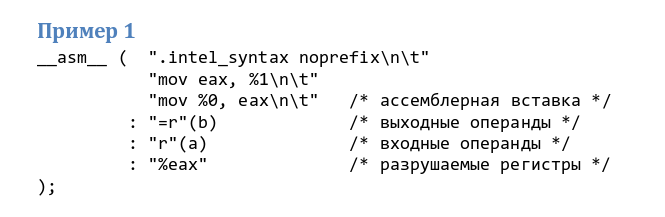
\includegraphics[scale=0.75]{Selection_069.png} 
\end{flushleft}

Директива .intel\_syntax меняет  синтаксис AT\&T на синтаксис Intel;  необходимо дополнительно указывать смену синтаксиса для операндов инструкций, \textbf{noprefix}, что позволит писать код в более близком к диалекту nasm виде, не используя при записи имен регистров префикс %. 
Допустима сокращенная версия вставки, состоящая только из строки с командами: 
\begin{flushleft}
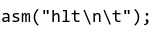
\includegraphics[scale=0.6]{Selection_070.png} 
\end{flushleft}
Для связи ассемблерных инструкций с переменными Си-программы используются следующие за вставкой два элемента оператора: списки операндов, в которых операнды перечислены через запятую. Каждый описанный операнд затем может использоваться в ассемблерных инструкциях, обращение к нему осуществляется по номеру с префиксом \%. Нумерация начинается с 0, и идет 
непрерывно, объединяя все элементы списков выходных и входных операндов.
1. Напишем простую программу для сложения двух чисел, с использованием ассемблерной вставки
\begin{minted}{c}
int main(void)
{
  int foo = 10, bar = 15;
  __asm__ __volatile__("addl  %%ebx,%%eax"
                       :"=a"(foo)
                       :"a"(foo), "b"(bar)
                       );
  printf("foo+bar=%d\n", foo);
  return 0;
}
\end{minted}
Здесь мы настраиваем GCC для записи значения из переменной foo в регистр \%eax, а bar в \%ebx, а результат будет в регистре \%eax. Знак ’=’ указывает, что это выходной регистр. 

2. Теперь рассмотрим более сложную, но полезную функцию. \\

\textbf{Копирование строки}. \\
\begin{minted}{c}
static inline char * strcpy(char * dest,const char *src)
{
int d0, d1, d2;
__asm__ __volatile__("1:\tlodsb\n\t"
                     "stosb\n\t"
                     "testb %%al,%%al\n\t"
                     "jne 1b"
                     : "=&S" (d0), "=&D" (d1), "=&a" (d2)
                     : "0" (src),"1" (dest) 
                     : "memory");
return dest;
}
\end{minted}
 Адрес источника записывается в esi, приёмника - в edi, а затем начинается копирование. Когда мы считываем 0, копирование завершается. Ограничители "\&S", "\&D", "\&a" указывают, что регистры esi, edi и eax являются ранними используемыми регистрами, то есть их содержимое будет изменено перед завершением функции. Здесь также понятно, почему память в списке используемых.\\

\textbf{Вывод}\\

В результете выполнения работы я узнал, как осуществляются ассемблерные вставки в языки высокого уровня, реализовав две простые программы на языке С, наглядно демонстрирующие работу с ассемблером. Таким образом, цель работы достигнута.

\par\bigskip
\textbf{Список используемой литературы}:
\begin{enumerate}
\item \url{http://av-assembler.ru/asm/high-level-languages/assembler-gcc.php} - Встроенный ассемблер GCC
\item \url{http://www.ibiblio.org/gferg/ldp/GCC-Inline-Assembly-HOWTO.html} \\ - GCC-Inline-Assembly-HOWTO
\item \url{http://asmcourse.cs.msu.ru/} - Архитектура ЭВМ и язык ассемблера
\end{enumerate}
\end{document}

